\section{Common base}
Figure 10.1 shows a bias techniques named common base bias.
Calculate the values of \(I_E\), \(I_B\), \(I_C\), and \(V_{CE}\). Then simulate the circuit to double-check your theoretical calculations.
Assume the current gain coefficient \(\beta = 100\).

\begin{figure}[ht]
    \centering
    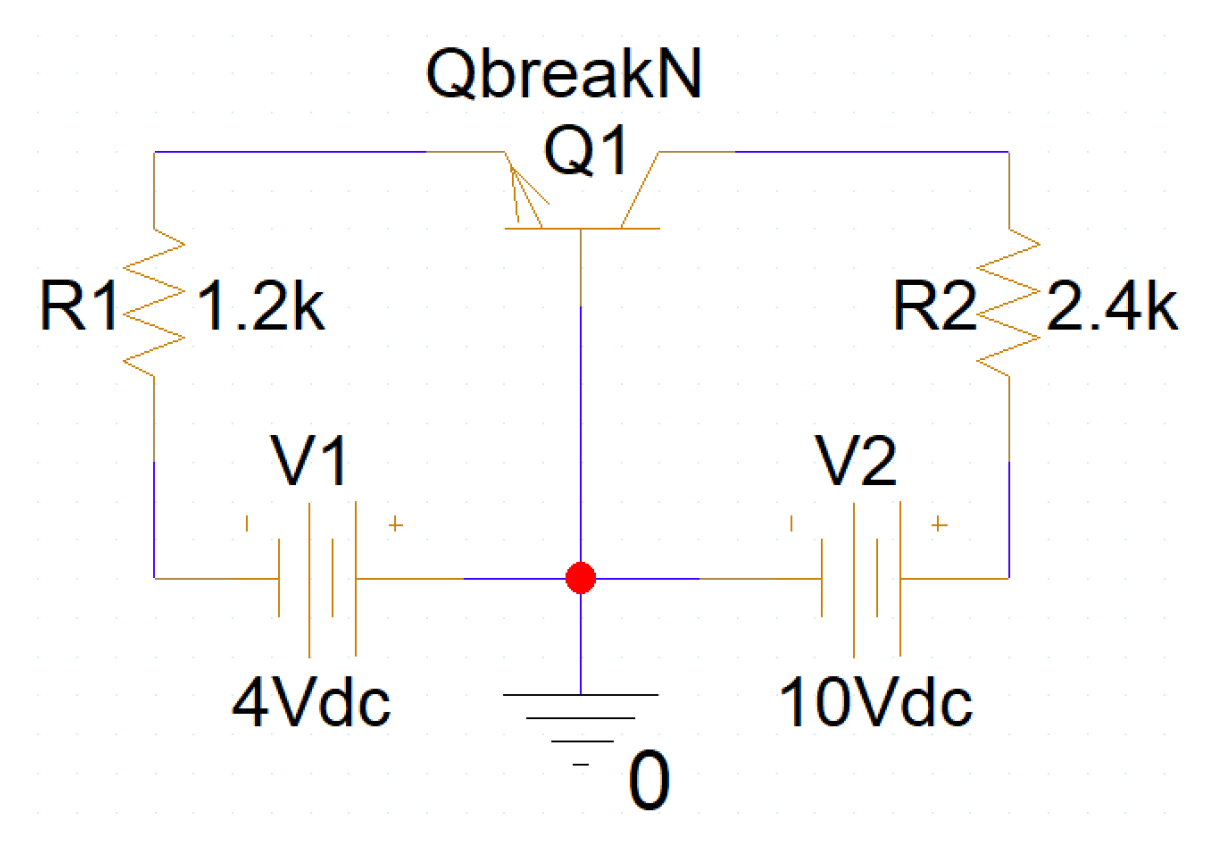
\includegraphics[scale=0.3]{graphics/ex10/f1.png}
    \caption{Common base}
\end{figure}
\subsection{Tính toán lý thuyết}
\textbf{Ghi chú:}

\textit{Những giải thích, công thức và phương trình được mong đợi hơn là chỉ có kết quả.}

Giả sử BJT trong vùng tích cực, ta có \(V_{BE} \approx 0,7\) (V)

\begin{figure}[ht]
    \centering
    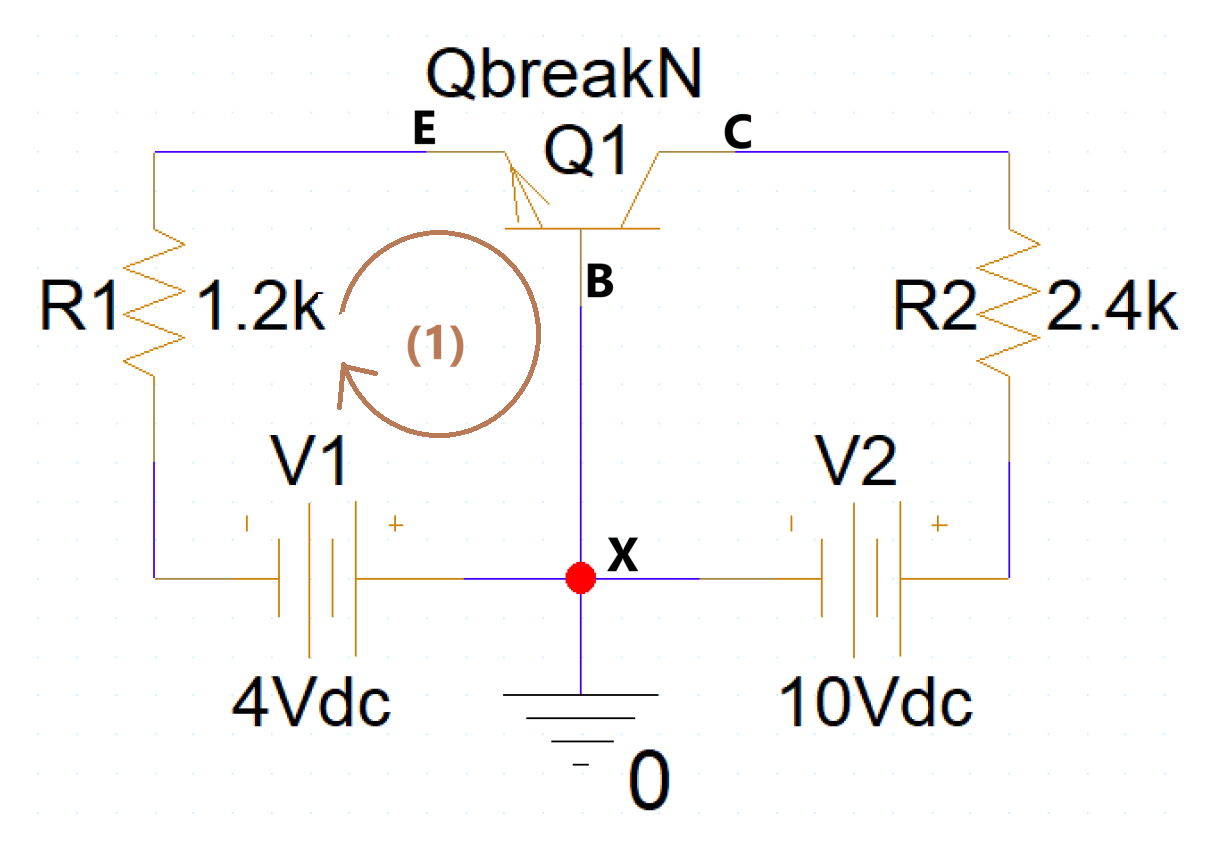
\includegraphics[scale=0.3]{graphics/ex10/f2.png}
    \caption{Common base}
\end{figure}

Theo KVL tại vòng (1), ta có:

\(V_1 - I_{E}R_1 - V_{BE} = 0 \iff 4 - I_{E}.1,2.10^3 - 0,7 = 0\)

\(\iff I_{E} = 2,75 (mA)\)

Theo KCL tại \(Q_1\), ta có: \(I_E = I_B + I_C\)

Mà \(I_C = \beta I_B = 100I_B\)

\(\iff I_E = 101I_B = 2,75\)

\(\iff I_B = \frac{2,75}{101} \approx 0,0272 (mA)\)

\(I_C = 100I_B \approx 2,723 (mA) \)

Theo KVL tại vòng lớn của mạch, ta có:

\(V_1 + V_2 - R_2I_C - V_{CE} - R_1I_E = 0 \iff V_{CE}= 4 + 10 - 2,4.2,723 -1,2.2,75\)

\(\iff V_{CE} = 4,1648 (V)\)

\subsection{Mô phỏng}

\begin{figure}[ht]
    \centering
    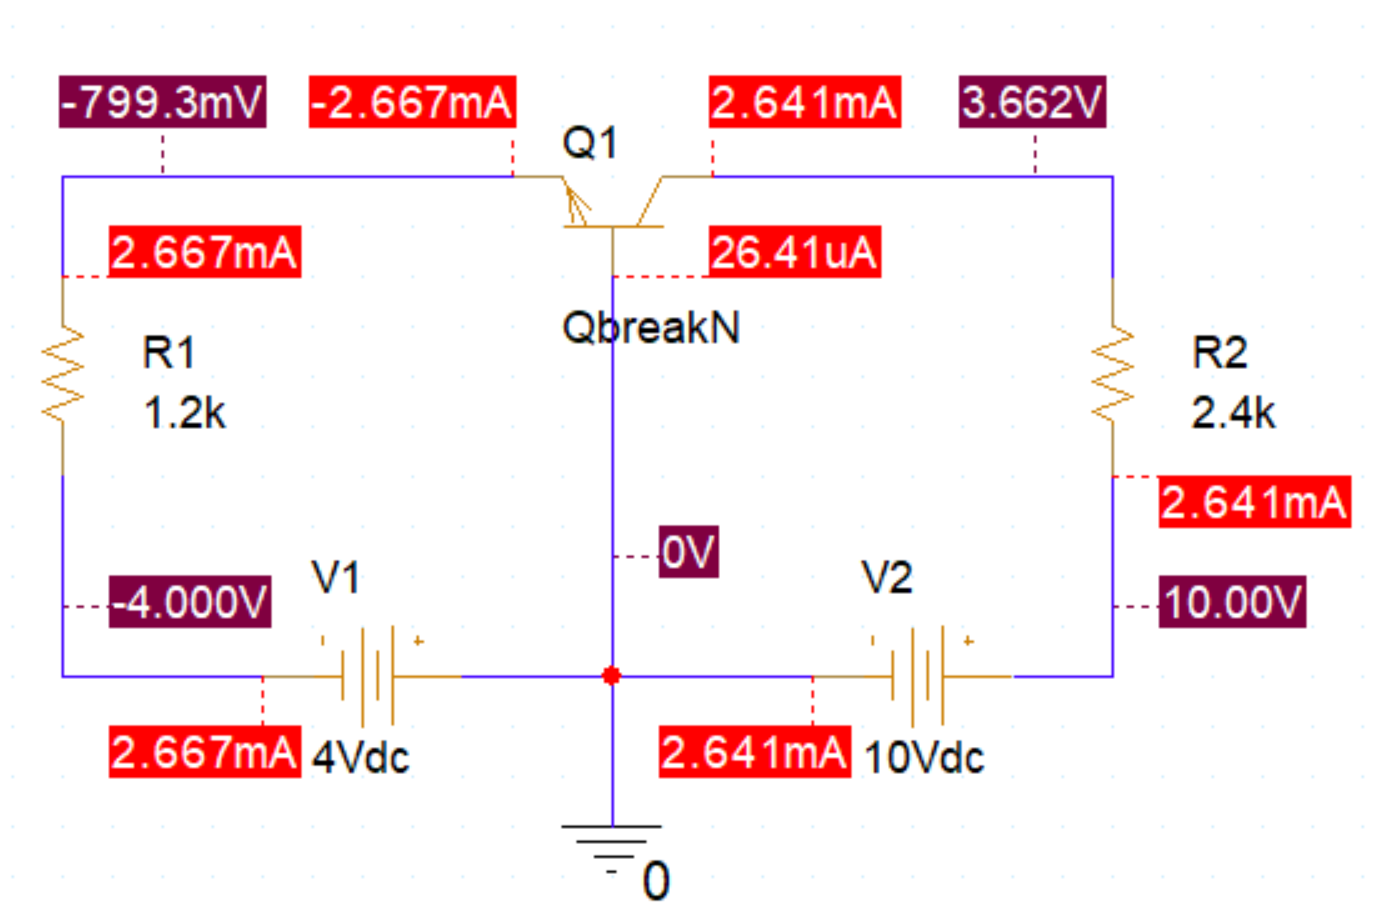
\includegraphics[scale=0.33]{graphics/ex10/f3.png}
    \caption{Simulation common base}
\end{figure}

Do ta giả sử \(V_{BE} \approx 0,7 \) V trong khi mô phỏng \(V_{BE} \approx 0,799 \) V nên kết quả mô phỏng có sự trên lệch so với tính toán lí thuyết.
\pagebreak
